\chapter{Robots}
A robot is a programmable, multifunctional machine designed to perform tasks by sensing its environment, processing information, and taking action either autonomously or semi-autonomously.



\section{Sensors}
    \subsection{IMU}
        IMUs come with 6 axis or 9 axis. 6 axis includes accelerometer and gyroscope and 9 axis also includes magnometer
        
        \subsubsection{Accelometer}
            To measure the x,y,z acceleration
        
        \subsubsection{Giroscope}
            to measure rotational rate, eitrher (roll, yaw, pitch) or quaternion
        
        \subsubsection{Magnetometer}
            It measures earth magnetic field. the output is a threed number
        
        \subsubsection{GPS}
        
        \subsubsection{LIDAR}
        
\section{Sense Plan Action loop}
    It is also called Perception-Planning-Control
    \begin{figure}[H]
        \centering
        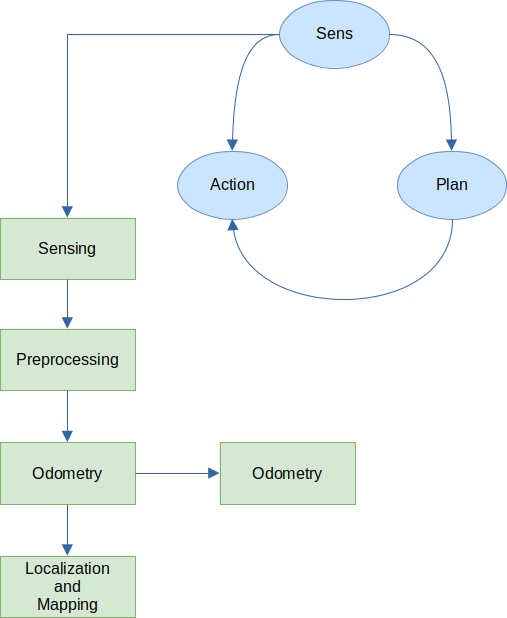
\includegraphics[width=0.8\linewidth]{/home/donkarlo/Dropbox/repo/phd_thesis/figs/sense_plan_act}
        \label{fig:my_png}
    \end{figure}
    
    \subsection{Sense}
        Perception has four layers
        \subsubsection{Sensing}
            Raw sensory data
        \subsubsection{Preprocessing}
        \subsubsection{Odometry and then State estimation}
            Odometry is the process of estimating a robot’s change in position (translation) and orientation (rotation) over time, using motion sensors.
        \subsubsection{Localication and mapping}
            \paragraph{SLAM}
                stands for simultanious localization and mapping. This is very related to self-awareness in a robot.
                    \subparagraph{Output}
                    SLAM output is  something like an ocuupancy grid
    
    \subsection{Plan}
        \paragraph{Goal} Goal is an input to planning
    \subsection{Action}
        Executes motor commands to follow the planned trajectory
            

\section{Action-Goal}
    A robot perform a set of actions to achieve a (set of) goals
    \paragraph{Action}
        Action is an assesable long running tasks such as goto point (x,y,z). Mavlink defines actions.
    \paragraph{Goal}
        A pose in which a robot should try to achieve
    \paragraph{Commands}
        instructions sent to actuators such as increase rotation speed of rotor 3 in a quadcopter

\section{The main components of a robot}:
The main components of a robot can be divided into five essential categories:

    \subsection{Physical components}
        \textbf{Sensors}: Allow robots to perceive both their environment and internal states, using sensors like cameras and LiDAR or IMUs.

        \textbf{Actuators}: Enable the robot to move or perform tasks by converting control signals into physical motion.
        Examples include motors, servos, robotic arms, and wheels.

        \textbf{Power Supply}: Provides the energy needed to operate the sensors, actuators, and processing unit.
        Examples include batteries, solar cells, and fuel cells.

        \textbf{Mechanical Structure}: The physical frame or body of the robot that supports and integrates the other components.
        Examples include wheels, legs, manipulators, and drone frames.

    \subsection{Virtual components:}
        \textbf{Controller (Processing Unit)}: The "brain" of the robot that processes sensor inputs, makes decisions, and sends commands to actuators.
        Examples include microcontrollers, processors, and embedded systems.

        \textbf{Goals} A goal in robotics refers to a desired outcome or end state that a robot aims to achieve through its actions. Unlike tasks, goals are typically long-term and result-oriented, requiring the robot to plan, adapt, and choose appropriate tasks to reach the desired objective. Goals can be static or dynamic, depending on environmental changes or new information. In autonomous systems, goals often drive decision-making by determining which tasks to prioritize and how to allocate resources. In cognitive architectures, goal management is critical for enabling goal-directed behavior and learning from experience.
        




\section{Different robots}

    \subsection{Non-Intelligent Robots:} These robots operate based on pre-programmed instructions with limited or no adaptability to changing environments. Examples include automated assembly-line robots or simple vacuum robots. 

    \subsection{Intelligent Robots:} These robots are capable of perceiving their environment, reasoning, and making decisions autonomously, often using AI techniques like machine learning. Examples include humanoid robots, autonomous vehicles, or drones with adaptive navigation systems. 

        \textbf{Cognitive Robots:} A subset of intelligent robots, cognitive robots are designed to mimic human-like cognitive processes, such as reasoning, problem-solving, memory, and understanding intentions. They focus on emulating human intelligence and are often used for tasks requiring higher-order reasoning and natural interaction, such as social robots like Pepper. 

        \textbf{Cognitive dynamic robots}

        \textbf{Concinnous robots}
        Probably never achievable. Pain must reduce computation resources in robot.They probably can never answer the question "What burning feels like" from recognized patterns in their in sensory data in their memory. Another aspect of pain might be messiness of words or meanings as sensory patterns in their memory.

\section{Feedback system}

\section{Control theory}

\section{Sensors}
    \begin{itemize}
        \item proprioceptive and exteroceptive sensors?
        \item sensory data
        \item Are sensory data only for state estimation ?
    \end{itemize}

\section{State estimation}
    \subsection{Questions}
        \begin{itemize}
            \item Is relating current sensor data with previous control inputs to solve problem a kind of state estimation?
        \end{itemize}
    
\section{Goal}
    \todo{This part must go under sense-plan-action cycle}
    \paragraph{Homestatis and survival}
        Somehow must prove that without having a surviavl goal self aware ness is not possible
        
        The survival final goal is the only effort that turns a robots attention to itself.
        
        Obeying the human ruler is one surviavl skill because the human ruler may kill the robot


        
\section{Simulation}
    \subsection{ROS ecosystem}
    
    
    \subsection{ROS}
    
    
    \subsection{MAVROS}
    A layer over ROS
    
    
    \subsection{MAVLink}
    The language to establish communication between
    \begin{itemize}
        \item QGroundControl and (MAVROS-MAVLink)
        \item (MAVROS-MAVLink) and (Autopilot)
    \end{itemize}
    
    
    \subsection{QGround Control}
    
    
    \subsection{Flight controller}
    The hardware board that usually containes
    \begin{itemize}
        \item IMU
        \item barometer
        \item GPS
        \item microcontroller/CPU
        \item I/O ports
    \end{itemize}
    
    Here are sime examples
    \begin{itemize}
        \item Pixhawk
        \item Cube orange
        \item Holybro
    \end{itemize}
    
    
    \subsection{Autopilot}
    The software
    
    \subsubsection{PX4}
    
    \subsubsection{PX4mini}
    
    \subsubsection{Ardupilot}
    
\section{Quadcopter}
    \subsection{Homeostatis}
    This could be considered as the final goal of a robot. Even a robot which follows its human master, it is better to be regarded as something that follows its master orders in order not to be destroyed by it
    This will be very intresting. A flying quadcopter is very prone to crashing. That is why it is a very good subject for self-awarness studies
